\section{Results}

\subsection{Variation in thrombolysis use}

Thrombolysis use in the original data varied between hospitals (figure \ref{fig:observed_thrombolysis}), from 1.5\% to 24.3\% of all patients, and 7.3\% to 49.7\% of patients arriving within 4 hours of known stroke onset.

\begin{figure}
\centering
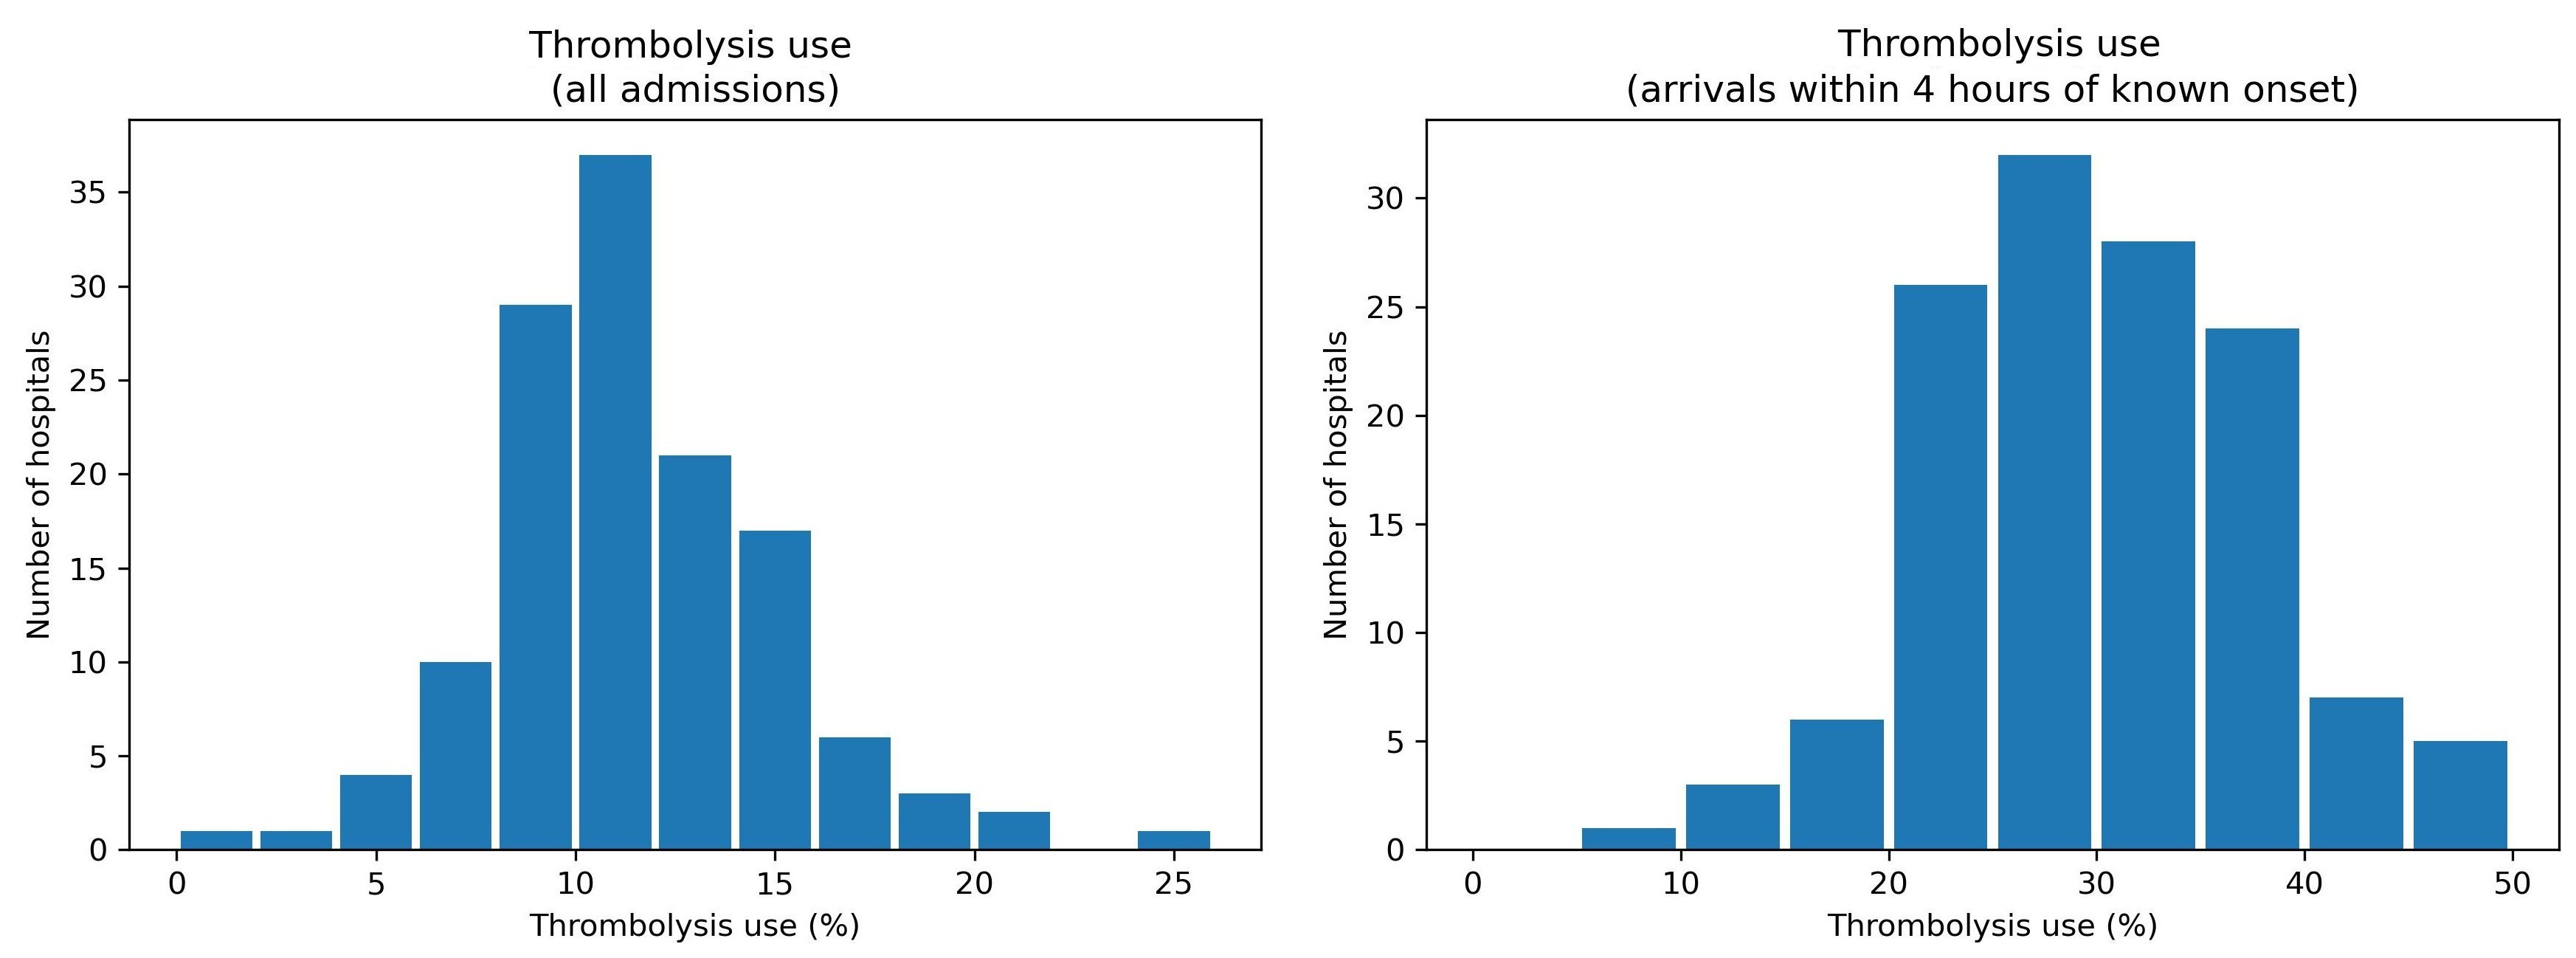
\includegraphics[width=1.0\textwidth]{./images/thrombolysis_hist}
\caption{Histogram of observed thrombolysis use in 132 hospitals. Left: Thrombolysis shown as a percentage of all emergency stroke admissions. Right: Thrombolysis shown as a percentage of those patients who arrive at hospitals within 4 hours of known stroke onset.}
\label{fig:observed_thrombolysis}
\end{figure}

\subsection{Feature selection}

In order to provide a more explainable machine learning model, the number of features were restricted to those that provide most information regarding use of thrombolysis. 25 features were selected by identifying one feature at a time that led to greatest improvement in Receiver Operating Characteristic (ROC) Area Under Curve (AUC). ROC AUC was measured using stratified 5-fold cross validation.

The best model with 1, 2, 5, 10, 25 \& all features (60 features before one-hot encoding of fields) had ROC AUCs of 0.715, 0.792, 0.891, 0.919, 0.923 \& 0.922. We selected 10 features for all subsequent work, which were:

\begin{itemize}
    \item \emph{Arrival-to-scan time}: Time from arrival at hospital to scan (mins)
    \item \emph{Infarction}: Stroke type (1 = infarction, 0 = haemorrhage)
    \item \emph{Stroke severity}: Stroke severity (NIHSS) on arrival
    \item \emph{Precise onset time}: Onset time type (1 = precise, 0 = best estimate)
    \item \emph{Prior disability level}: Disability level (modified Rankin Scale) before stroke
    \item \emph{Stroke team}: Stroke team attended
    \item \emph{Use of AF anticoagulants}: Use of atrial fibrillation anticoagulant (1 = Yes, 0 = No)
    \item \emph{Onset-to-arrival time}: Time from onset of stroke to arrival at hospital (mins)
    \item \emph{Onset during sleep}: Did stroke occur in sleep?
    \item \emph{Age}: Age (as middle of 5 year age bands)
\end{itemize}

Correlations between the 10 features were measured using coefficients of determination (r-squared). All r-squared were less than 0.15, and all r-squared were less than 0.05 except 1) age and prior disability level (r-squared 0.146), and 2) onset during sleep and precise onset time (r-squared 0.078). All correlations are shown in table \ref{tab:correl}.

\subsection{Model accuracy}

Model accuracy was measured using stratified 5-fold cross validation. Overall accuracy was 85.0\% (83.9\% sensitivity and specificity could be achieved simultaneously). The ROC AUC was 0.918. The model predicted hospital thrombolysis use at each hospital with very good accuracy (r-squared = 0.977).

The appendix contains further accuracy measures, and results for model validation of hospital thrombolysis curves, evaluation of variation in model prediction using bagging, learning rates, model calibration, and fine-tuning of model regularisation.

\subsection{Waterfall plots of SHAP values}

Waterfall plots show the influence of features for an individual prediction. We generally handle SHAP values as how they affect log odds of receiving thrombolysis, but for individual predictions, probability plots are more intuitive. The examples below are for a patient with low (top) and high (bottom) probability of receiving thrombolysis. The model starts with a base prediction of a 24\% probability of receiving thrombolysis, before feature values are taken into account. For the patient with a low probability of receiving thrombolysis, the two most influential features reducing the probability of receiving thrombolysis are a long arrival-to-scan time (138 minutes) and a low stroke severity (NIHSS=2). For the patient with a high probability of receiving thrombolysis, the two most influential features increading the probability of receiving thrombolysis are a short arrival-to-scan time (17 minutes) and a moderate stroke severity (NIHSS=14). 

\begin{figure}
\centering
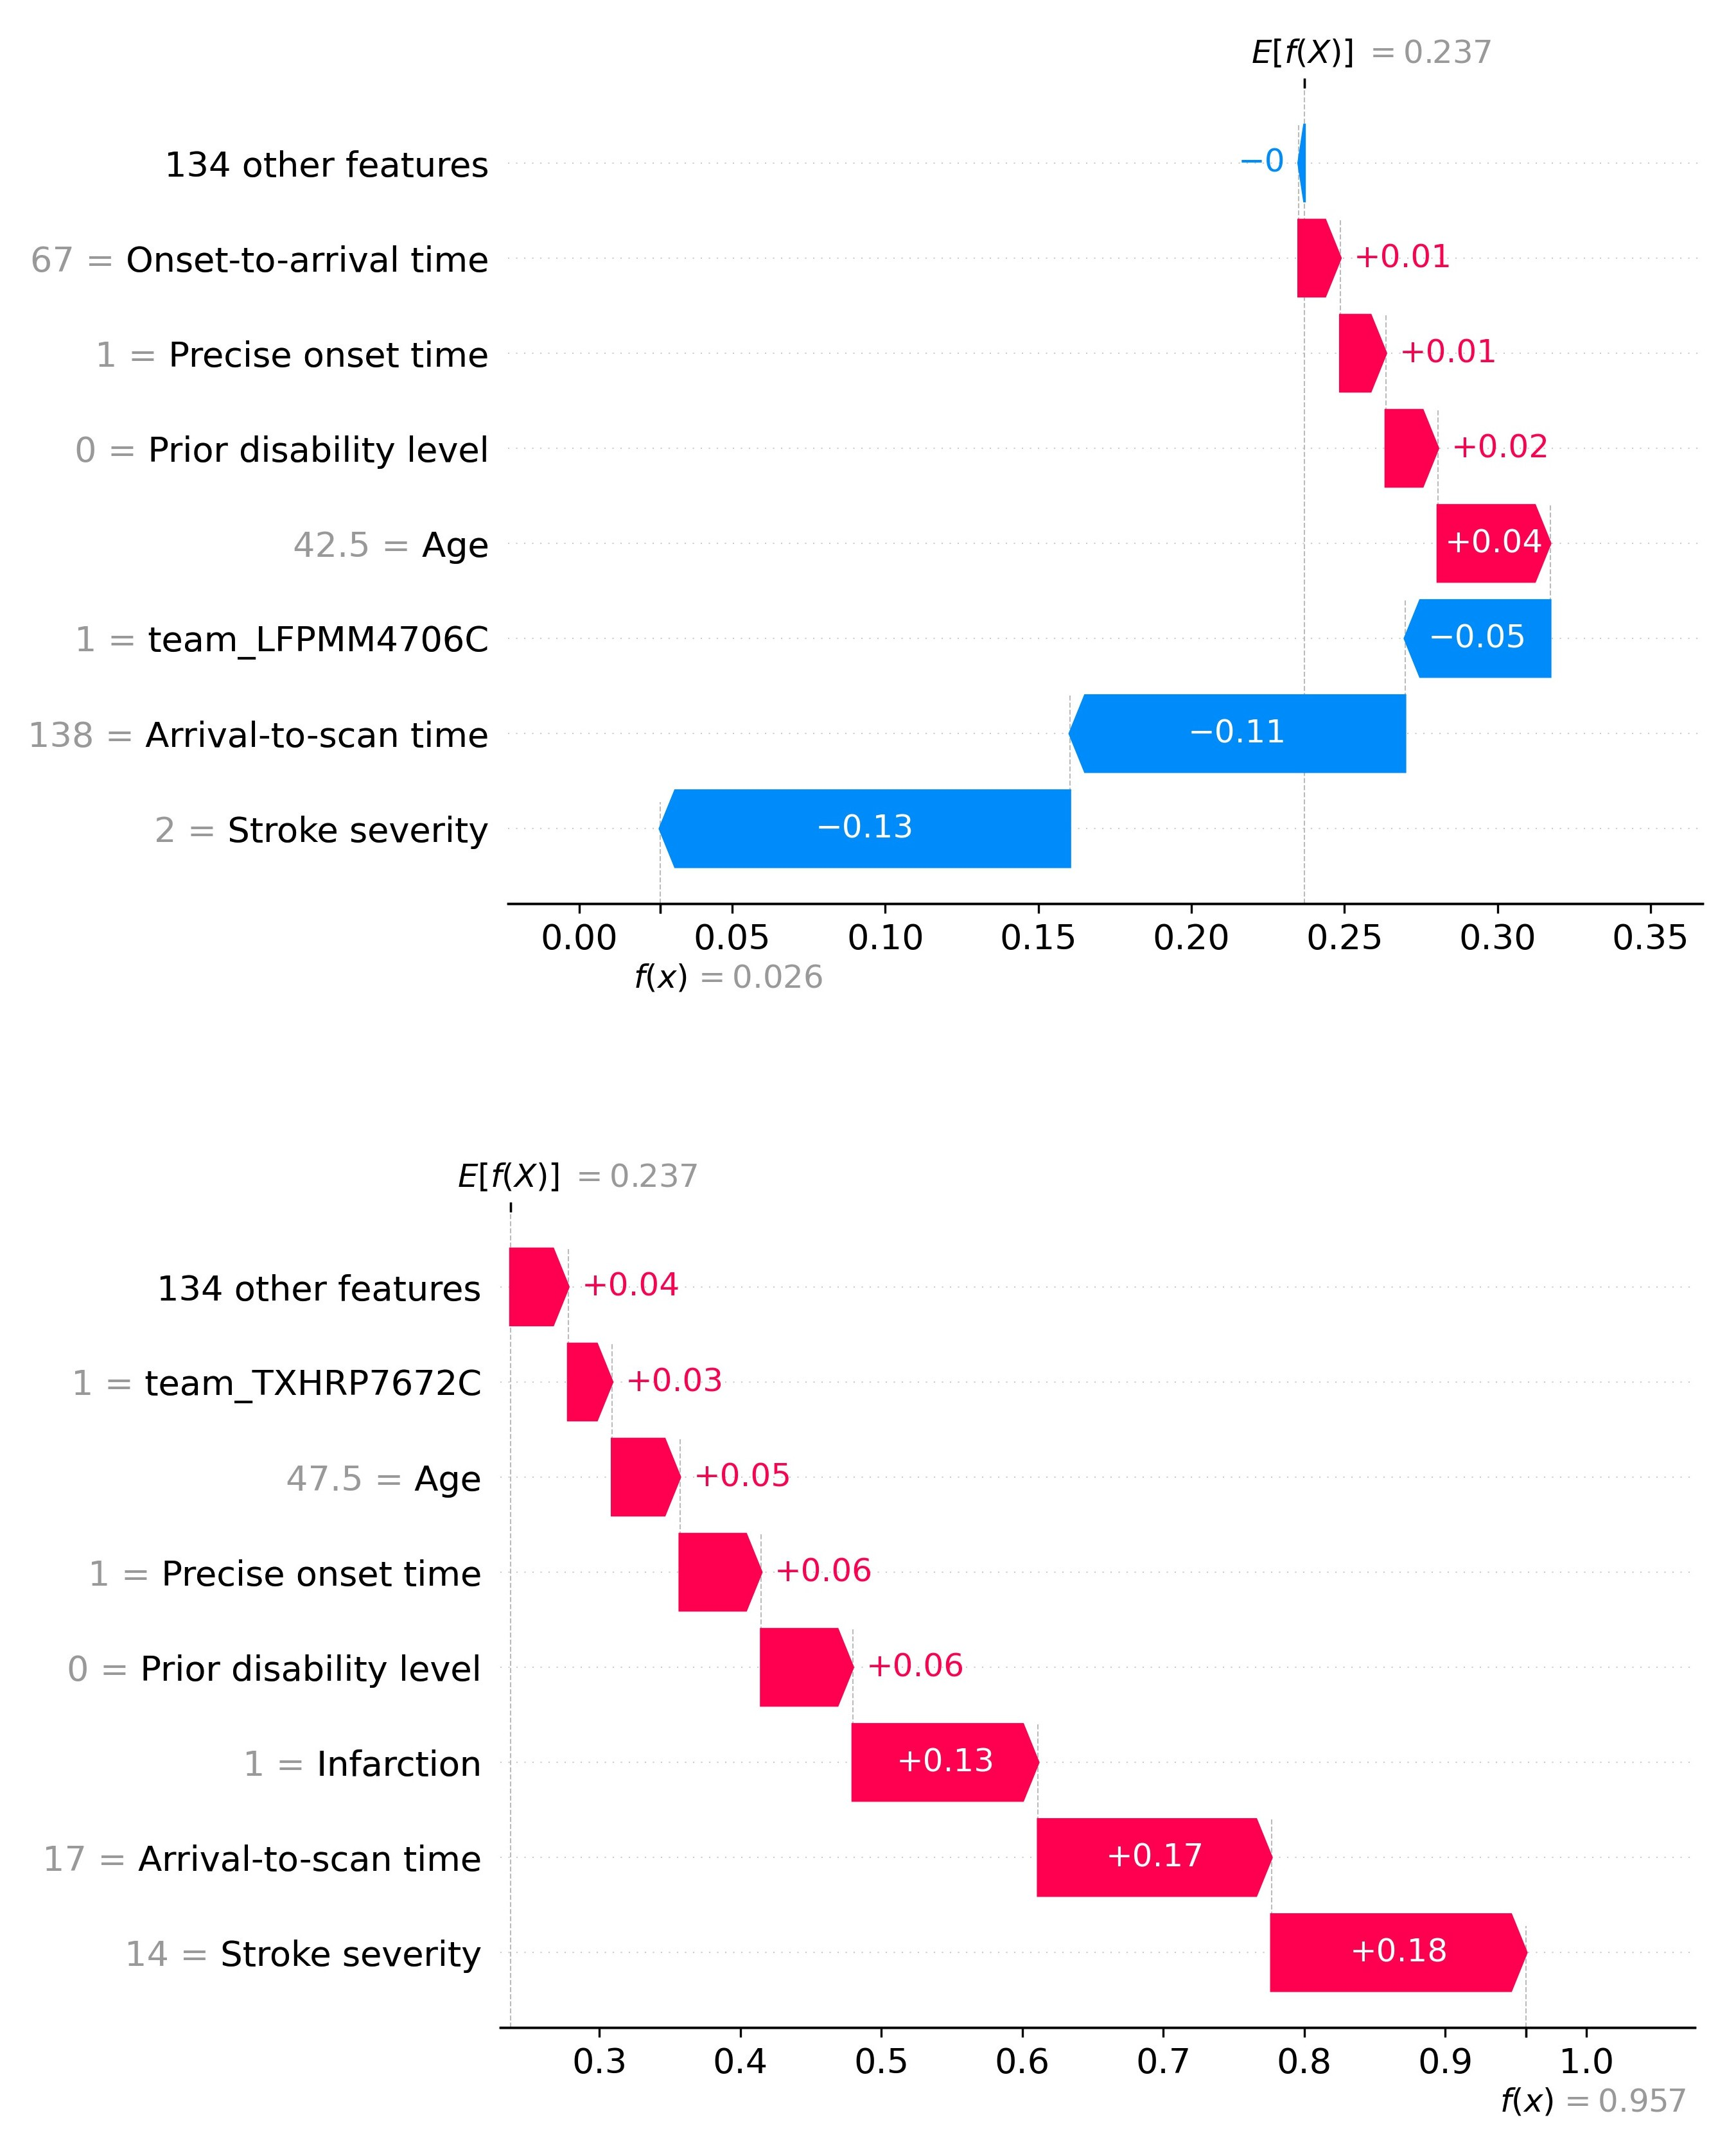
\includegraphics[width=0.8\textwidth]{./images/waterfall}
\caption{Waterfall plots showing the influence of each feature on the predicted probability of a single patient receiving thrombolysis. Top: An example of a patient with a low probability (2.6\%) of receiving thrombolysis. Bottom: An example of a patient with a high probability (95.7\%) of receiving thrombolysis.}
\label{fig:waterfall}
\end{figure}




\begin{figure}
\centering
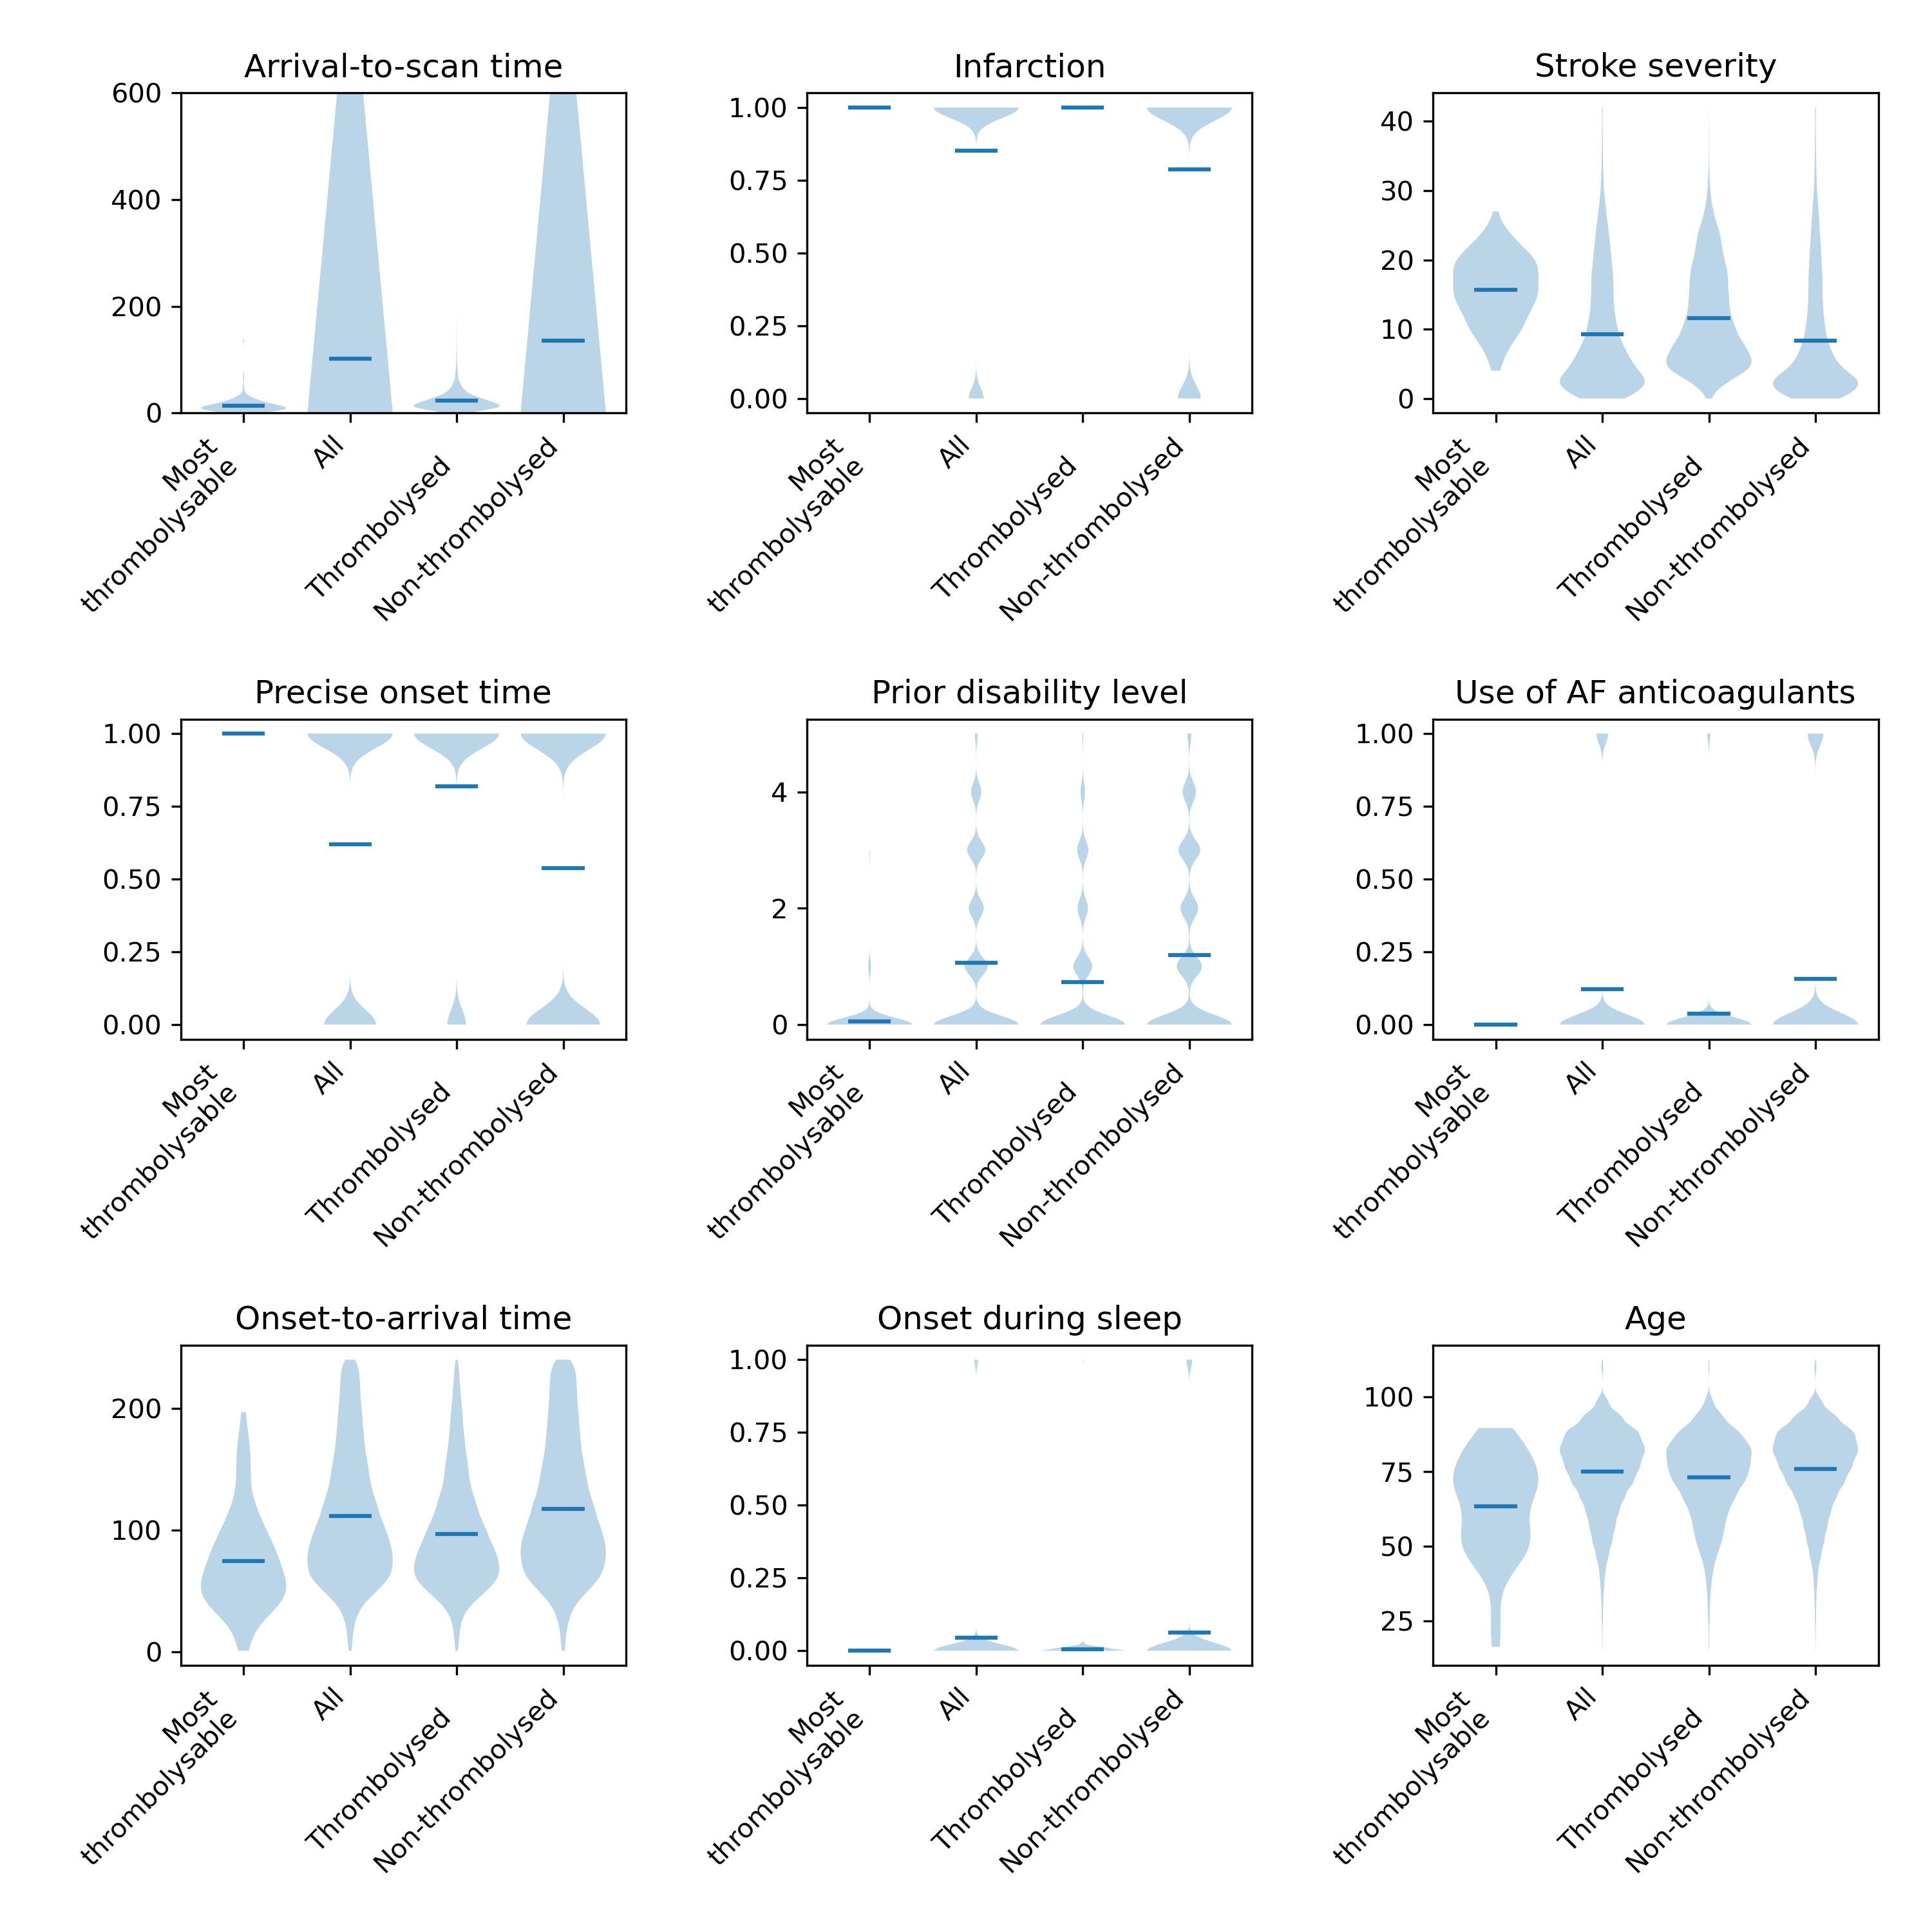
\includegraphics[width=0.8\textwidth]{./images/02a_most_thrombolsyable_violin}
\caption{Violin plots comparing feature values between the patient with the highest probability of thrombolysis at each hospital with all patients, all patients who had received thrombolysis, and all patients who had not received thrombolysis. Horizontal lines show the mean value of each group.}
\label{fig:waterfall}
\end{figure}


\begin{figure}
\centering
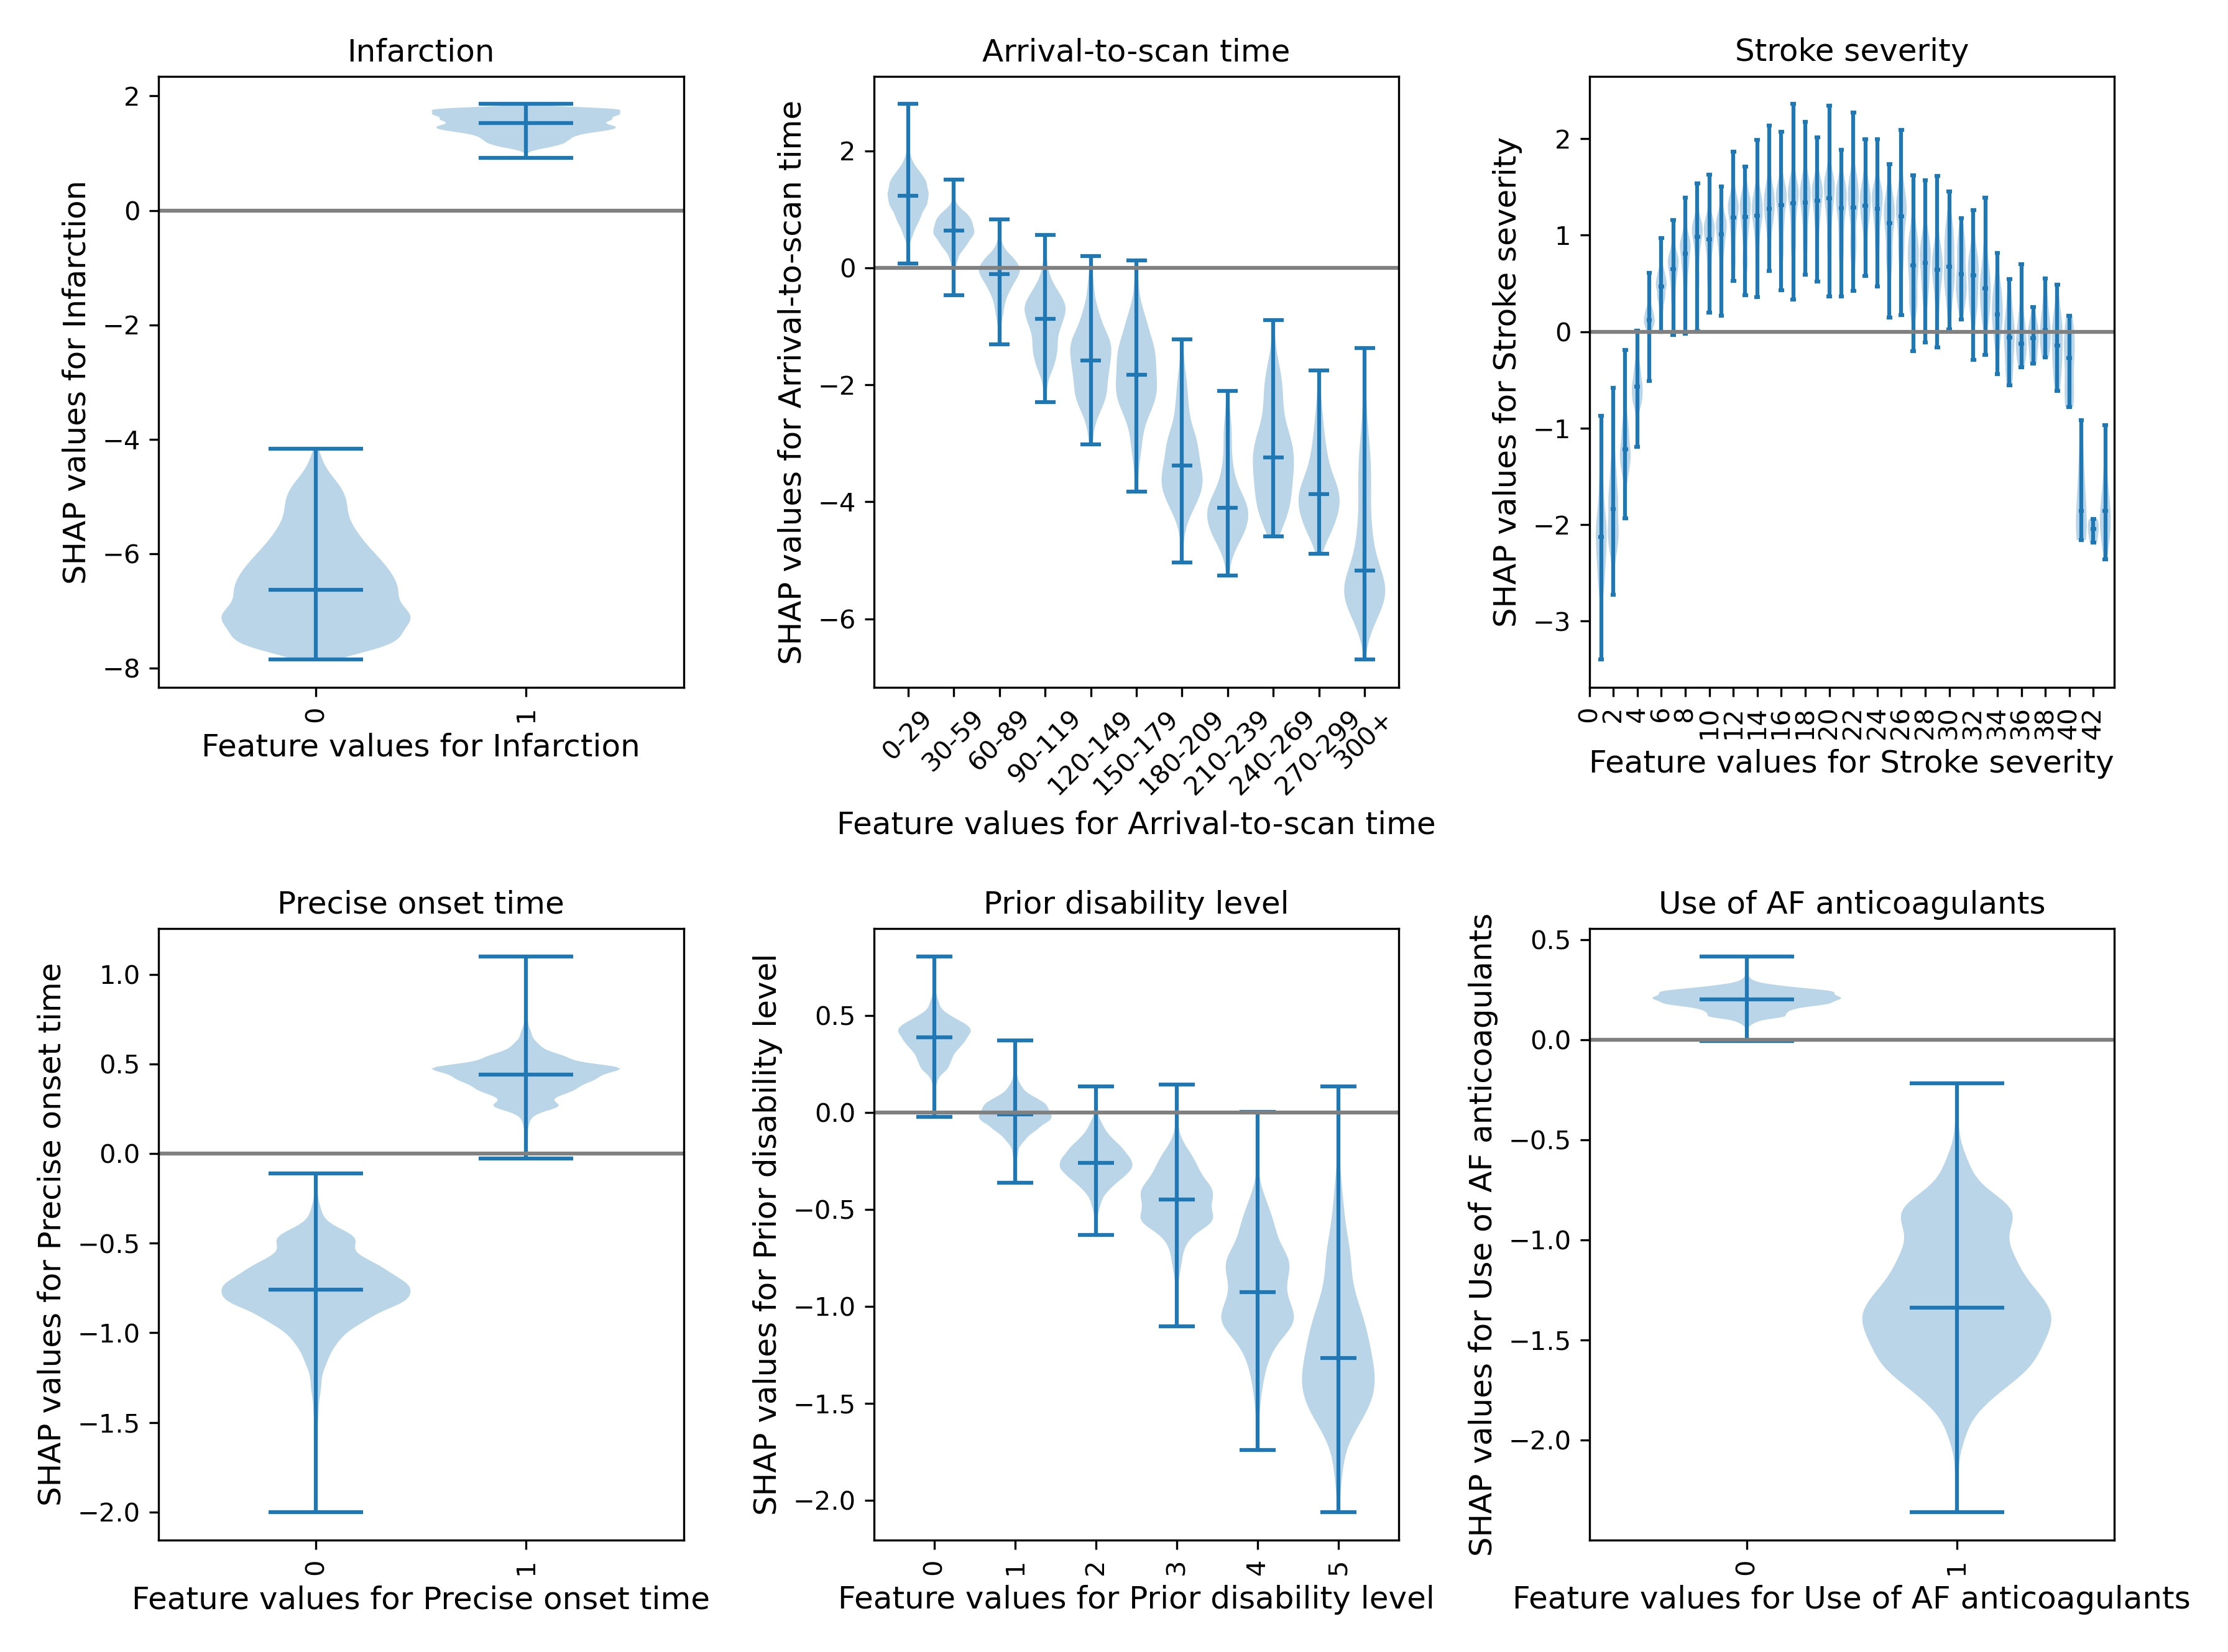
\includegraphics[width=1\textwidth]{./images/03_xgb_10_features_thrombolysis_shap_violin}
\caption{Violin plots showing the relationship between SHAP values and feature values. The horizontal line shows the median SHAP value. SHAP values were taken from the training set of the first of 5 k-fold train/test splits.}
\end{figure}

\begin{figure}
\centering
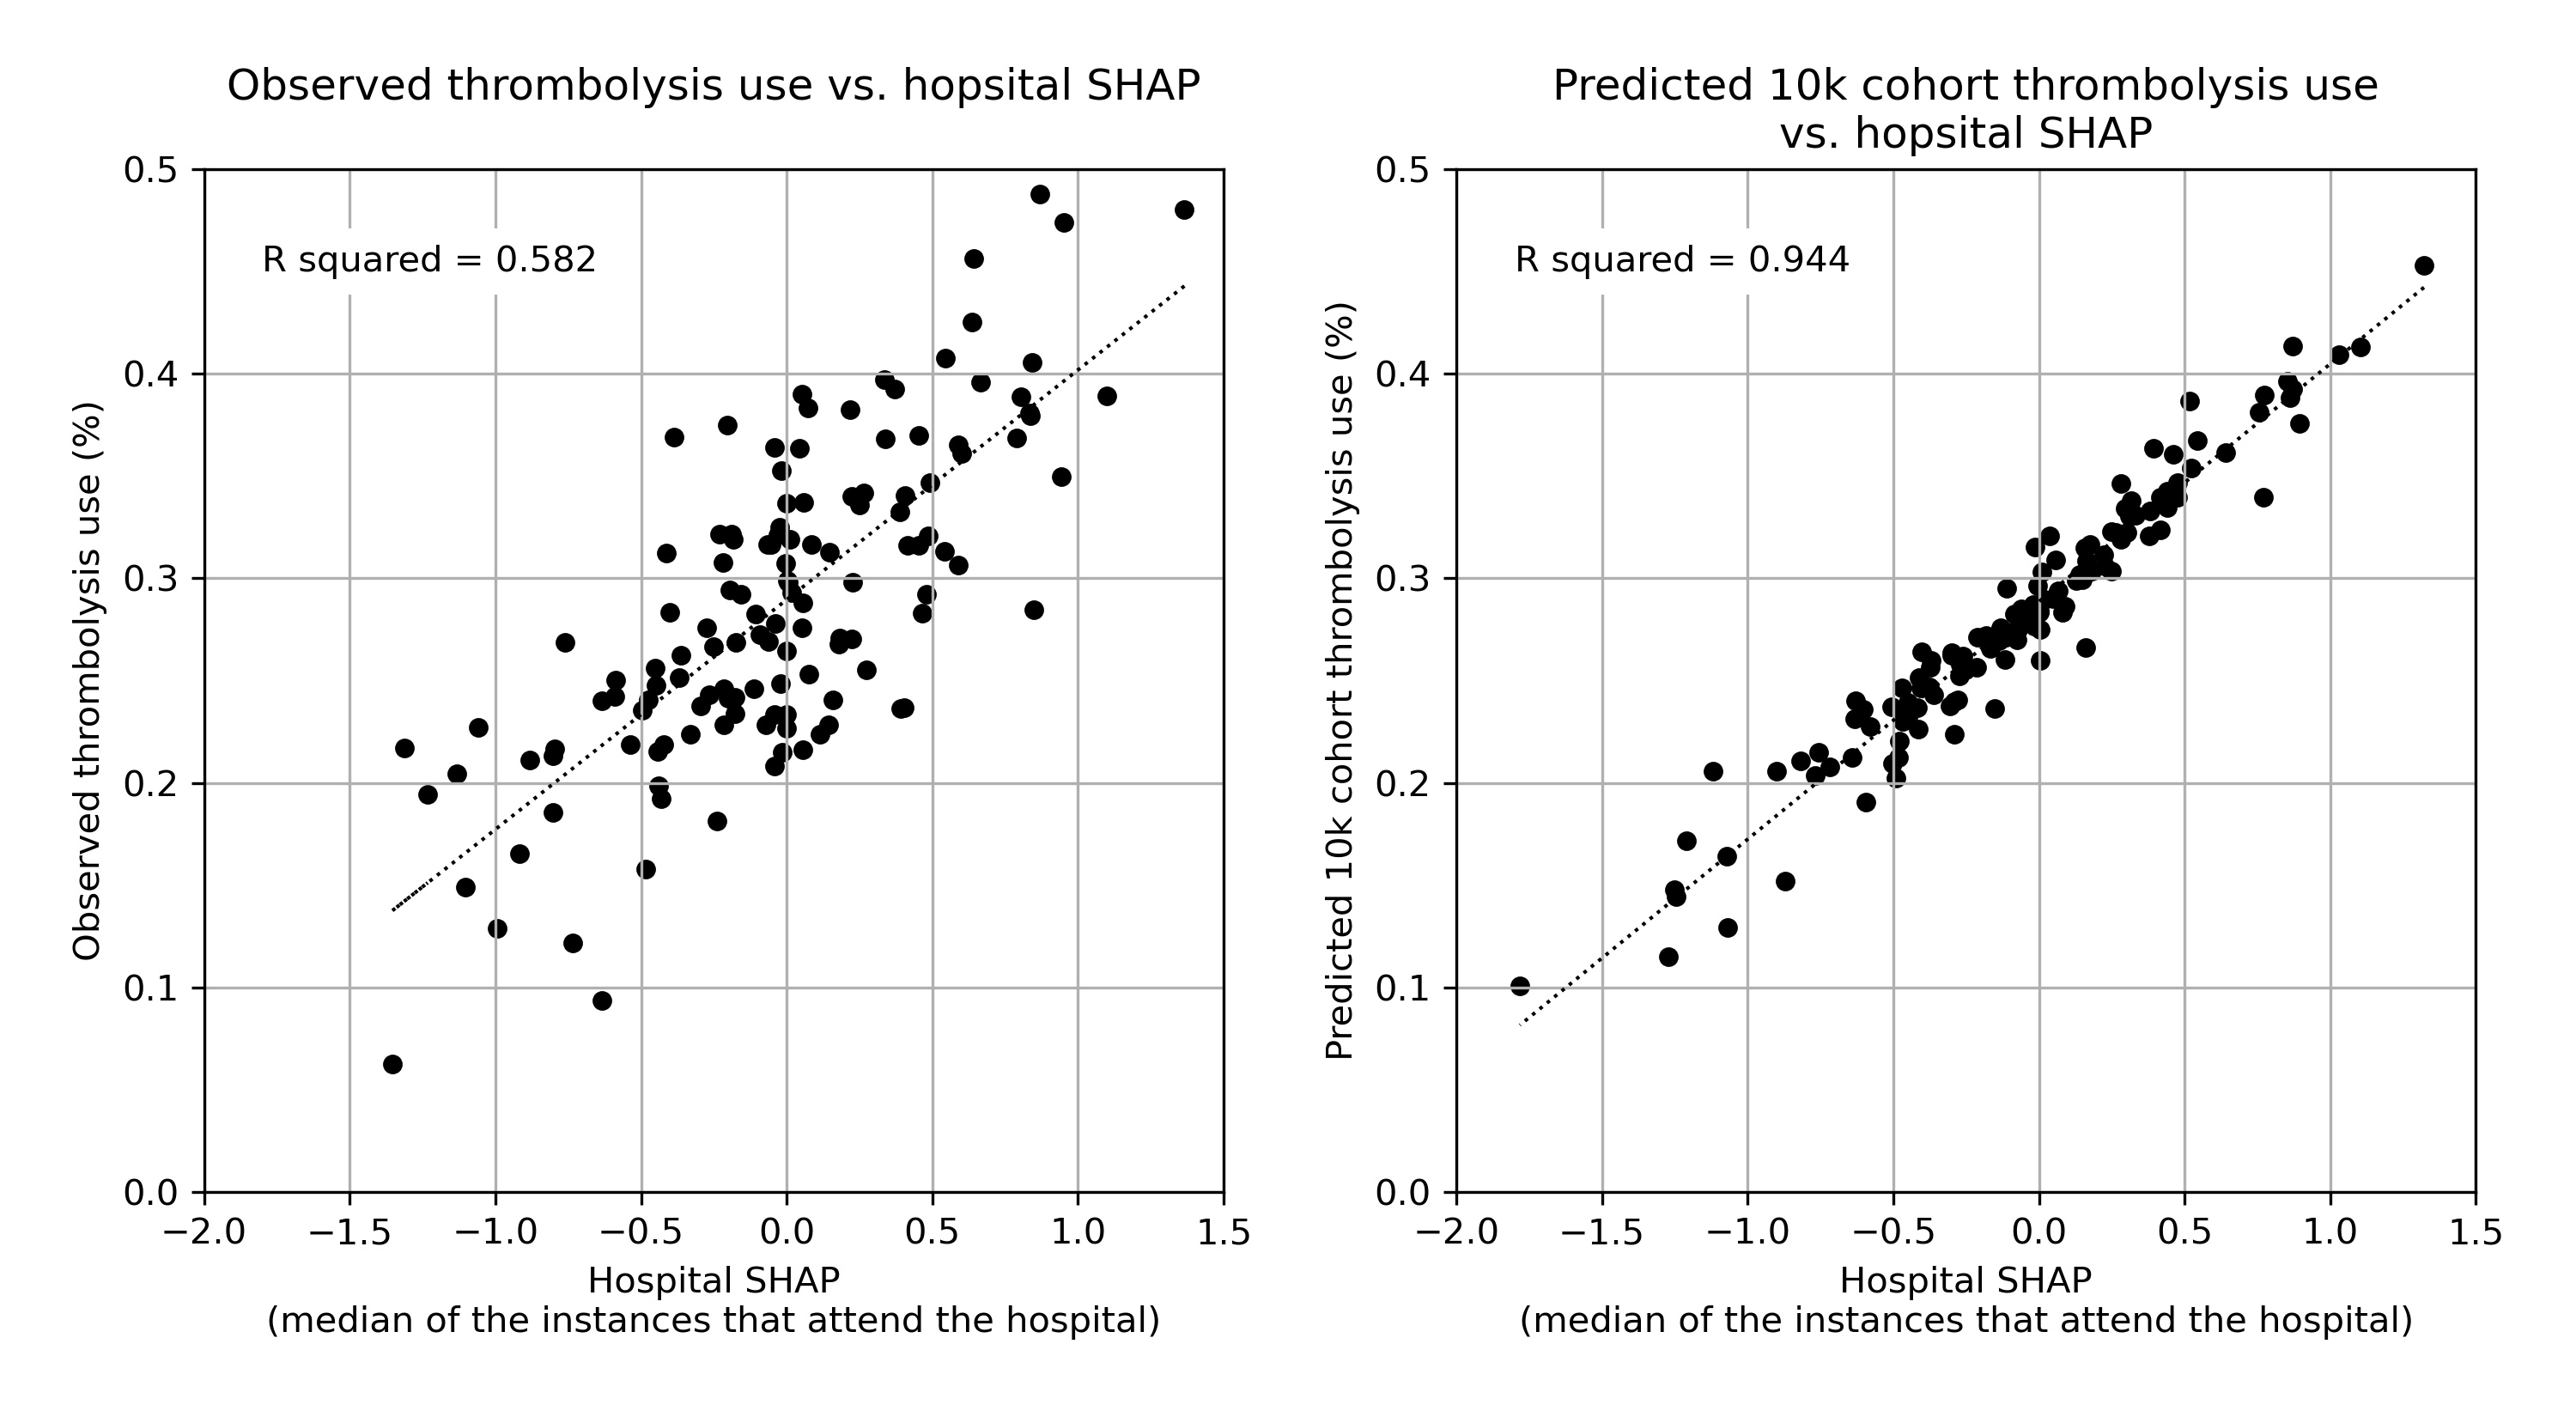
\includegraphics[width=1\textwidth]{./images/99_twin_correlation_scatter}
\caption{}
\end{figure}



\begin{figure}
\centering
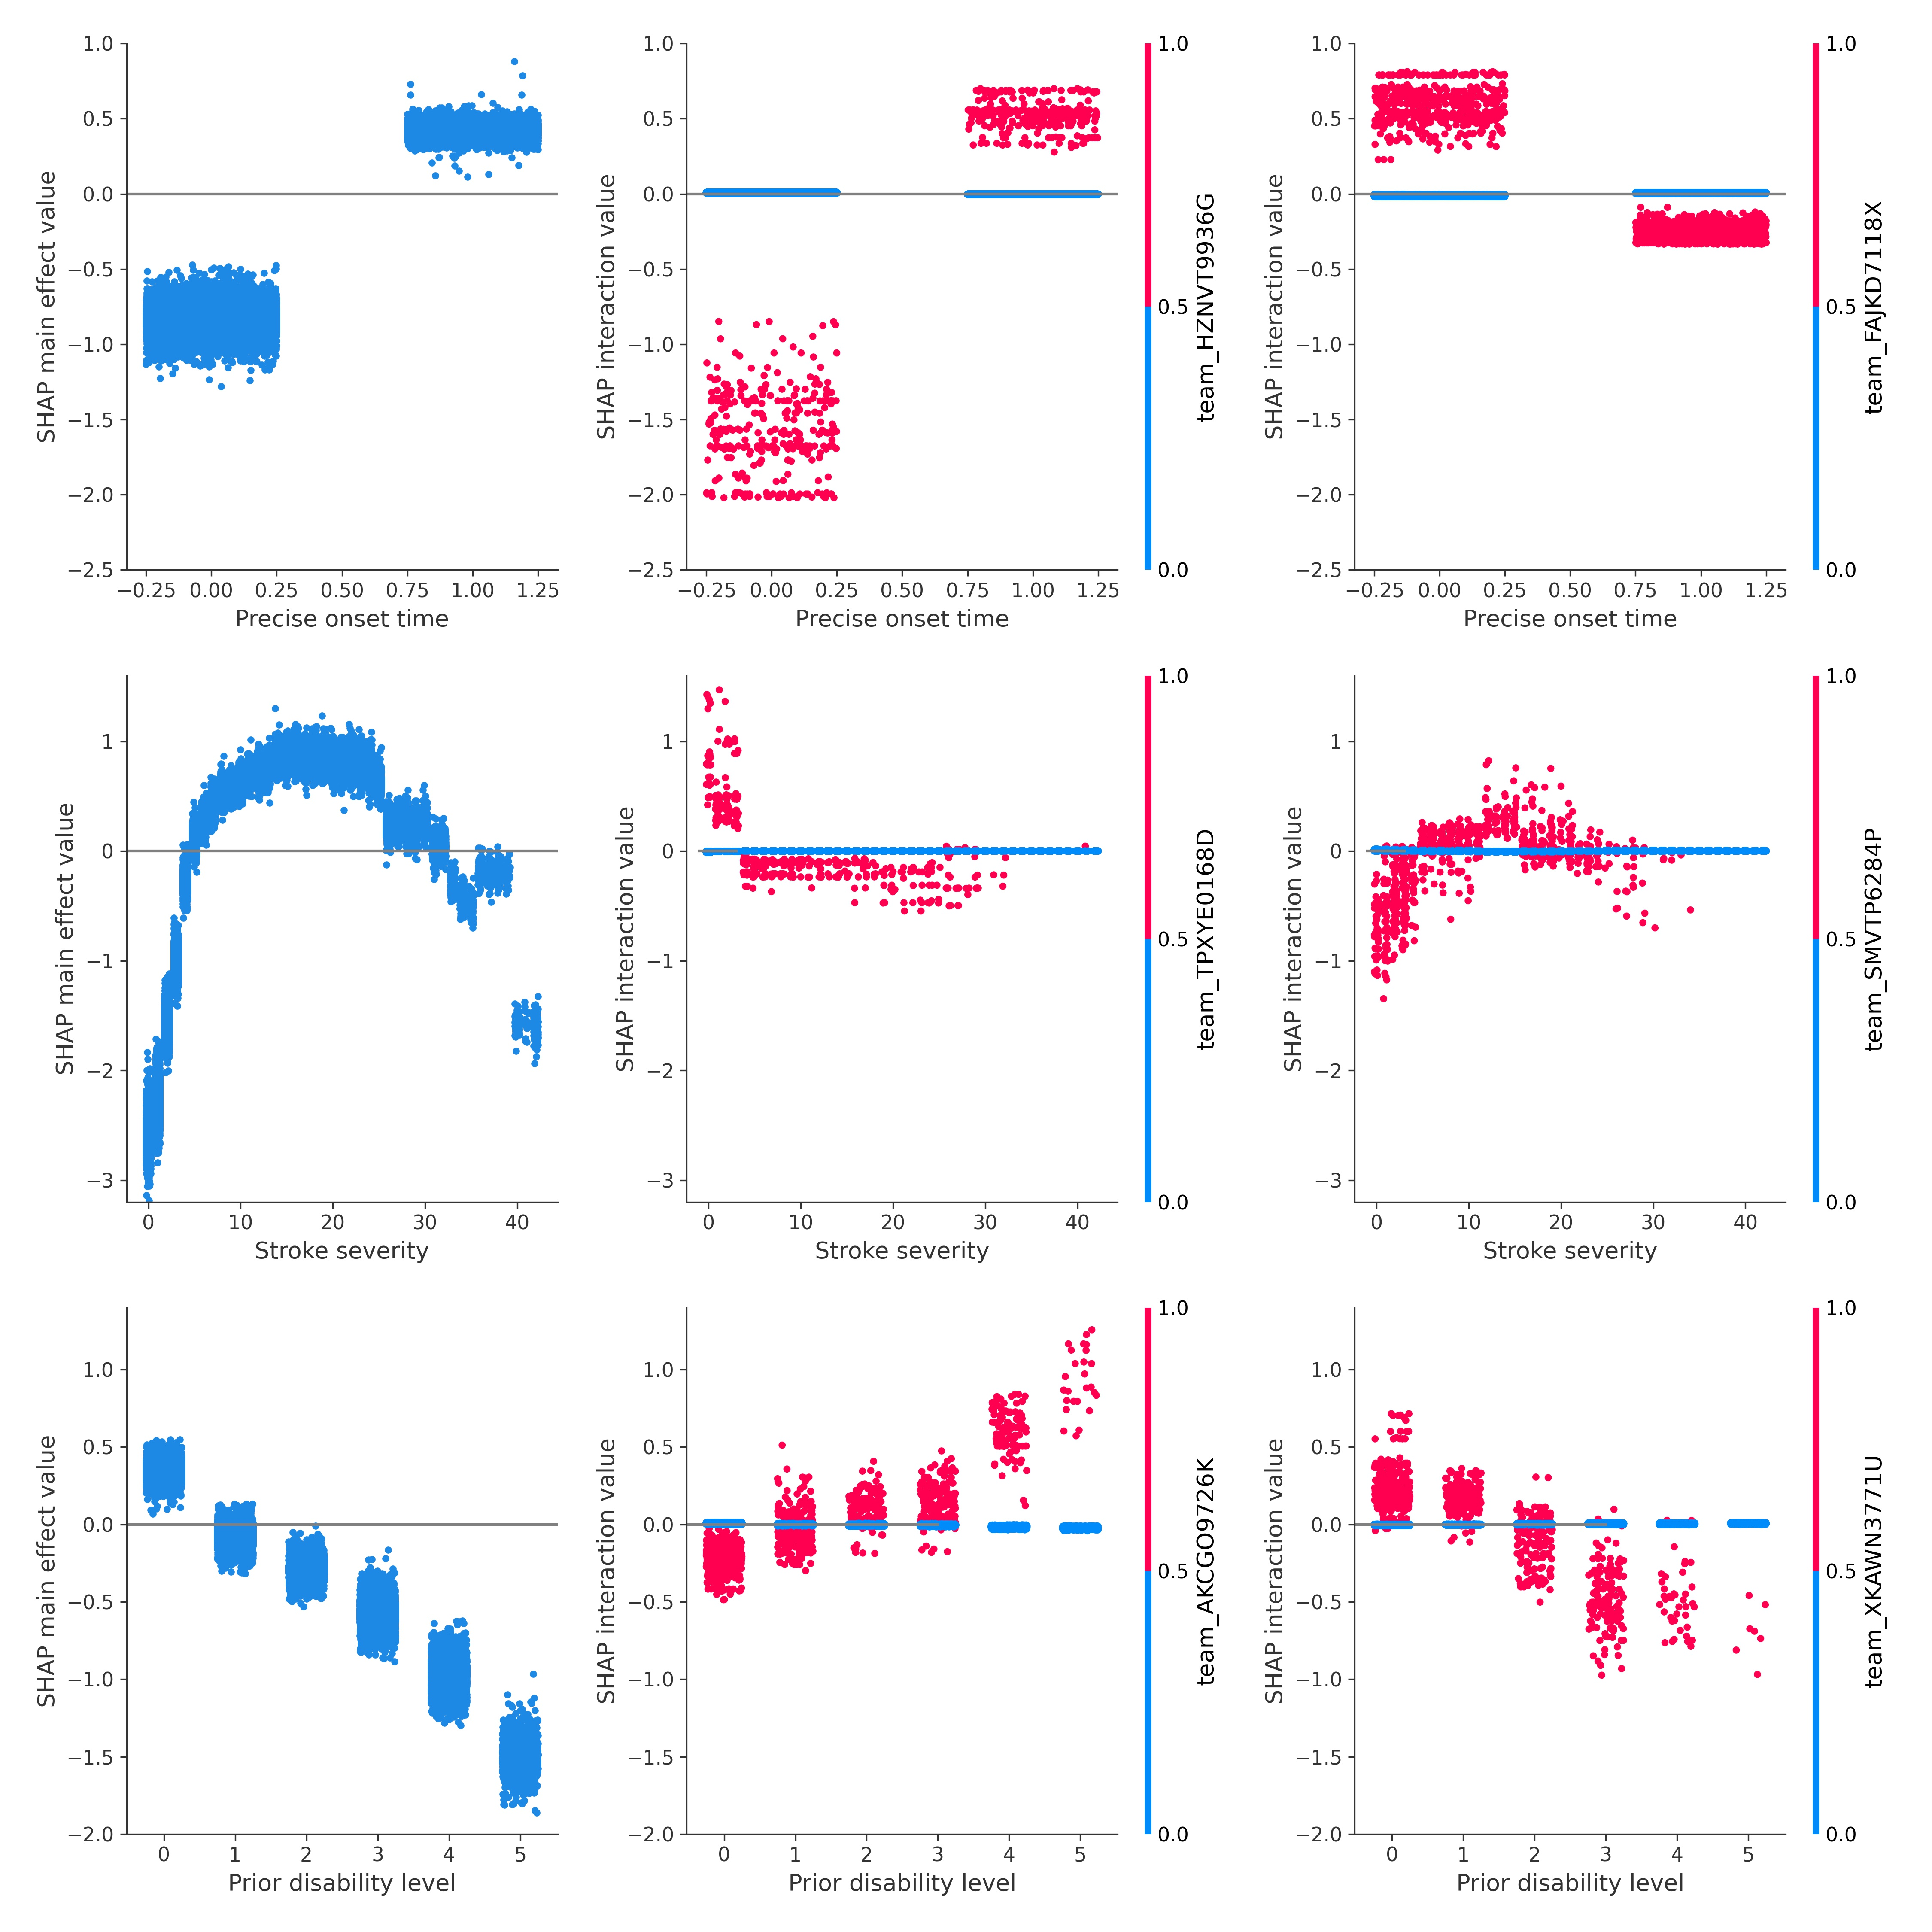
\includegraphics[width=1.0\textwidth]{./images/12aa_xgb_10_features_3_features_interaction_example_with_main_effect}
\caption{}
\end{figure}

SHAP interaction between hospital ID for two teams and whether stroke onset time was known precisely. If a patient attended team HZNVT9936G then SHAP value for having a precise onset time was increased (a strengthening of the main effect of precise onset time). If a patient attended team FAJKD7118X then SHAP value for having a precise onset time was reduced (an attenuation of the main effect of precise onset time).


\begin{figure}
\centering
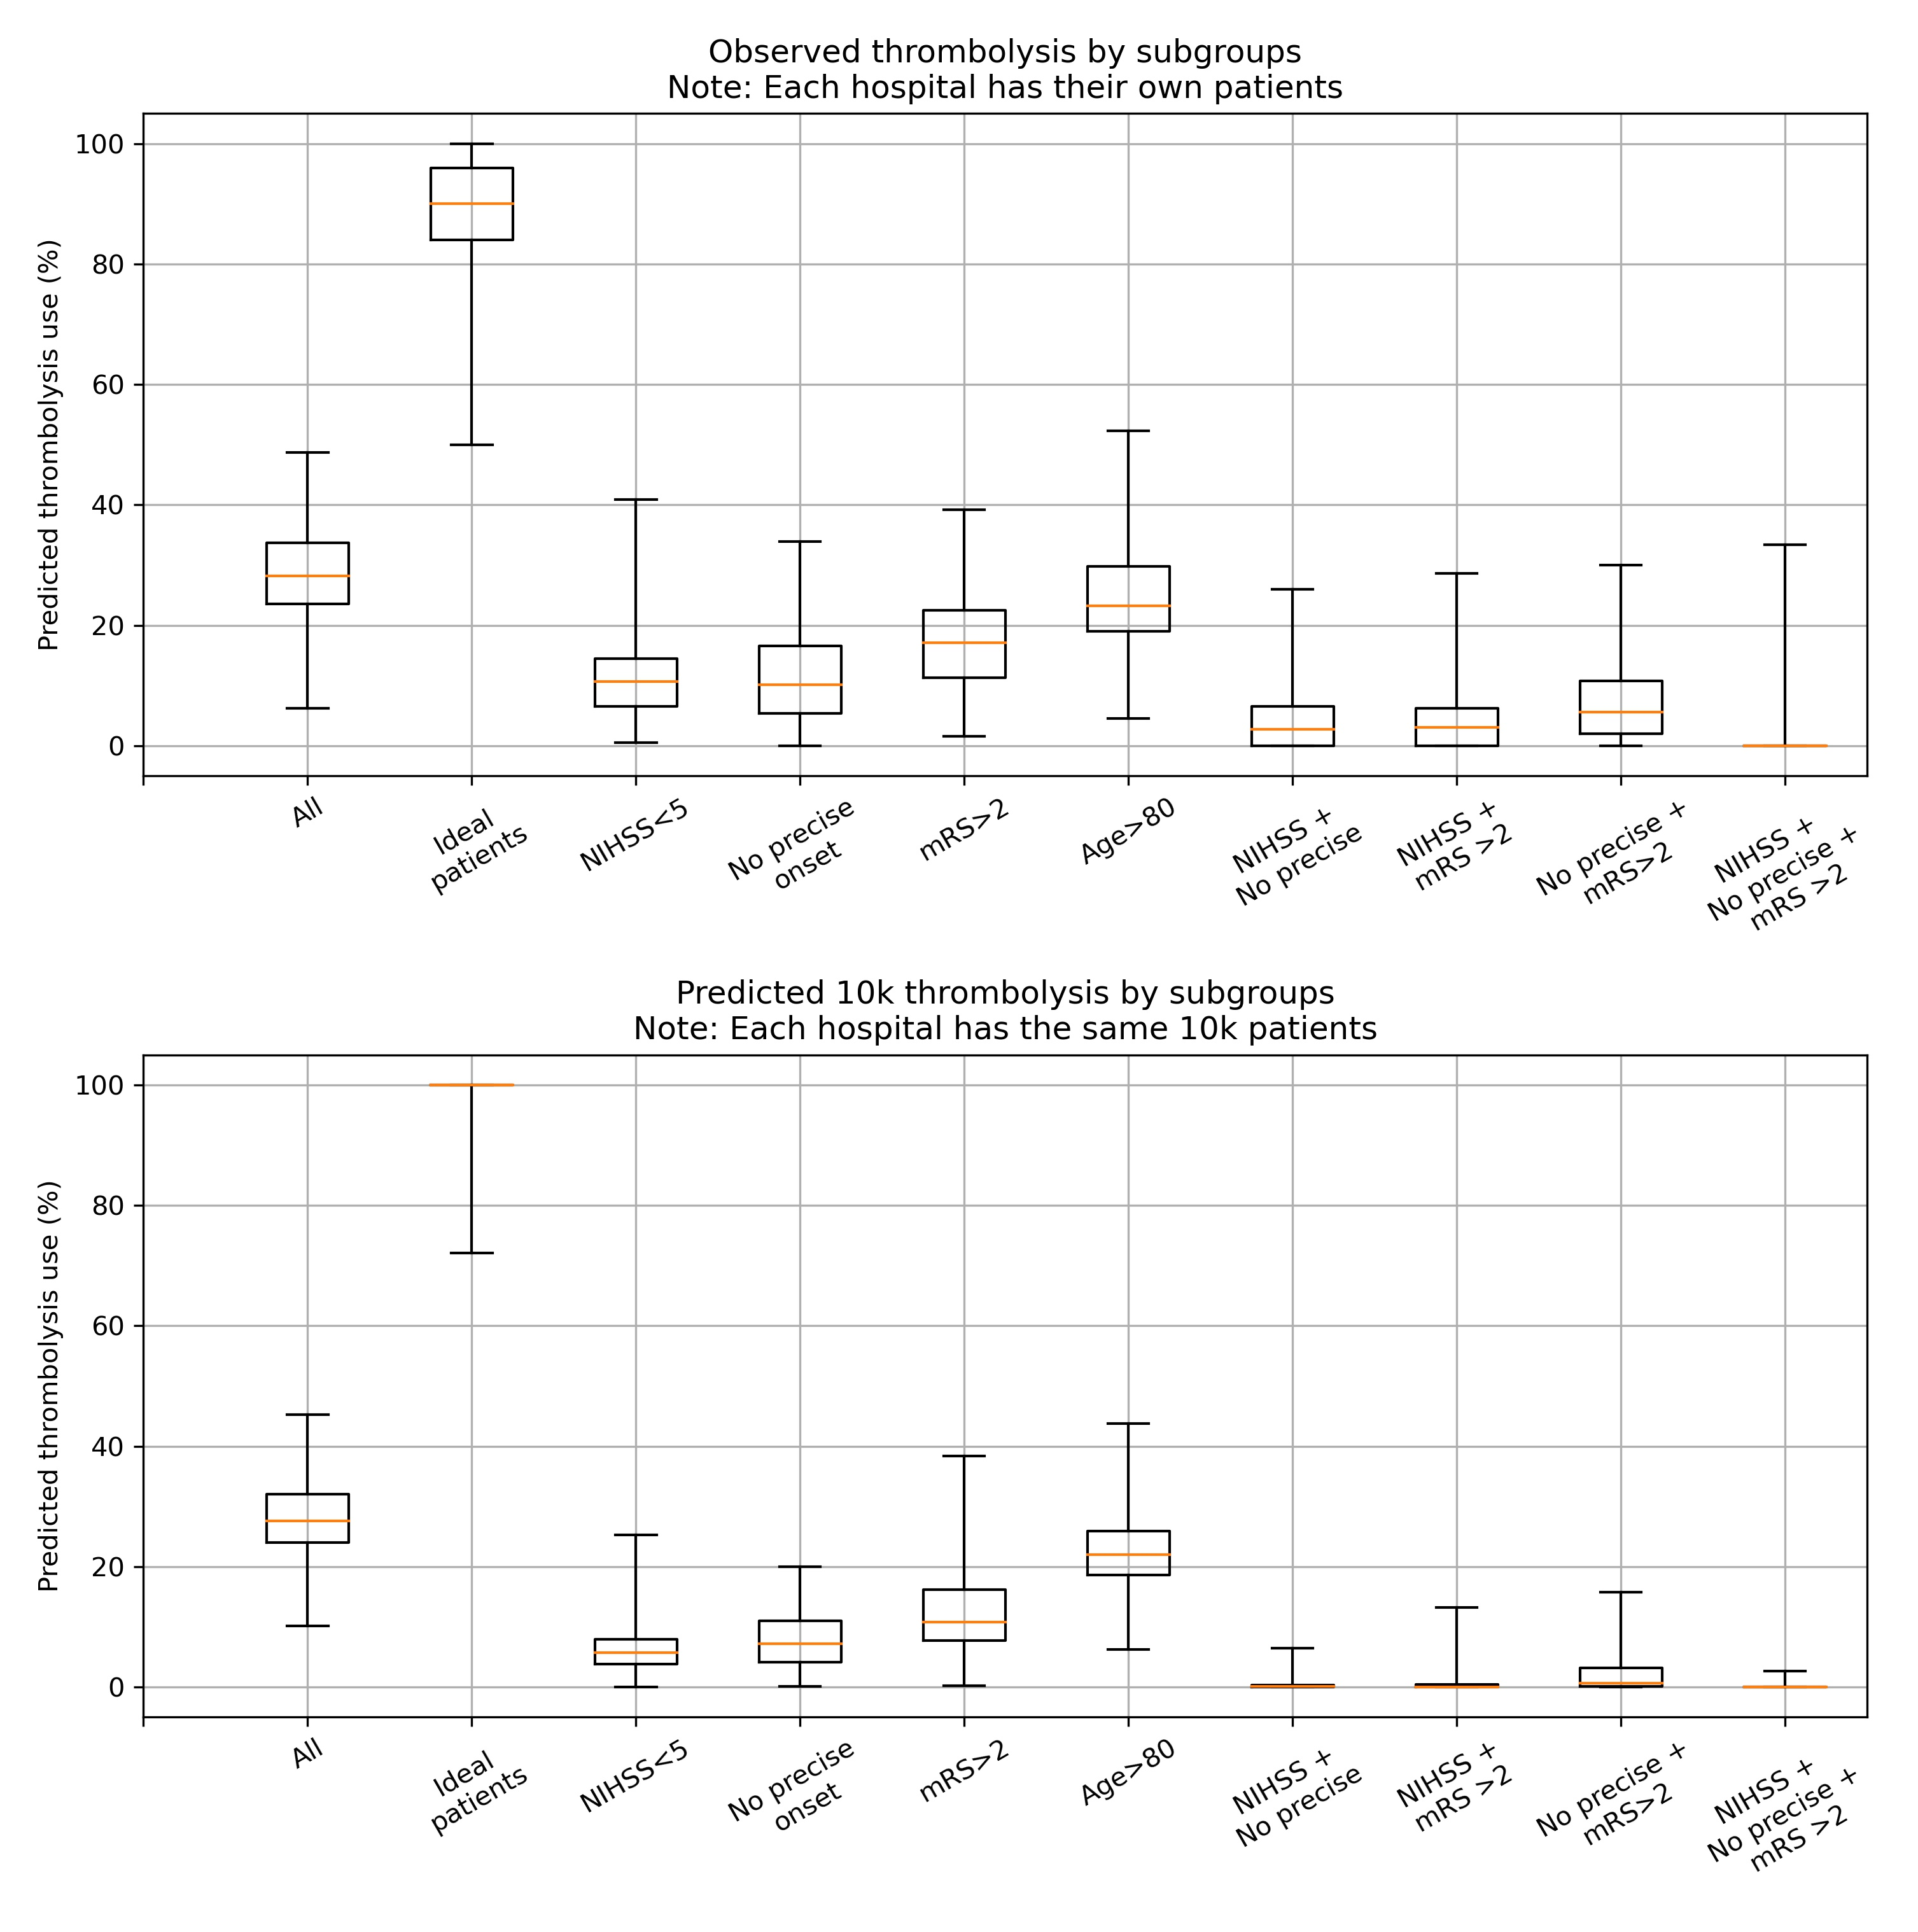
\includegraphics[width=1\textwidth]{./images/15a_actual_vs_modelled_subgroup_violin}
\caption{Boxplot for either observed (top) or predicted (bottom) use of thrombolysis for subgroups of patients.}
\end{figure}





% Add detail on how standard devisation chart binned









